** REMEMBER TEXT! **

\section{Pre-processing}
The data is pre-processed in MatLab where the pain maps are imported. To easier analyse the data afterwards all the images are converted into row vectors and then inserted into a single matrix. The pain maps are represented in three different data representations and therefore the pain maps are processed in three different ways before compiling all image-vectors in a matrix. 
The three data representations are a matrix consisting of the pain morphology, a matrix with only the knee regions that are covered in pain, and lastly a matrix consisting of both the pain morphology and the affected knee regions. 
To get additional information about the subjects and the associated pain maps, another input, gender, is added to the three matrices. This is done by including an extra column vector containing genders after the last column in each matrix. 
Furthermore, the three data representations have to be tested in neural network models with two different output parameters; duration of PFPS and pain intensity. The output parameters are, like gender information, added as column vectors to the matrices so that the neural network models can analyse the pain information, gender and either duration or pain intensity. Only one output parameter is added to each matrix, which results in six different matrices.

VI SKAL PÅ EN ELLER ANDEN MÅDE SKRIVE HVORFOR PAIN INTENSY ER 0,1 and 2!!!

\subsection{Morphology} \label{sec:Morph}
The first representation of data is a binary matrix of the original pain maps. 
Firstly, the image of the original pain map is gray-scaled to get a one-dimensional matrix instead of a three-dimensional RGB-matrix. This matrix is then converted into a matrix consisting of zeroes and ones, where the pain pixels are symbolized with ones. Afterwards the matrix is resized, since the given data was collected at different resolutions (screen sizes). Furthermore the matrix is cropped to sort out unnecessary data like the areas inferior and superior to the knee. An image consisting of a binary matrix is shown as figure \ref{fig:cropbin7}.

\begin{figure} [H]
\centering
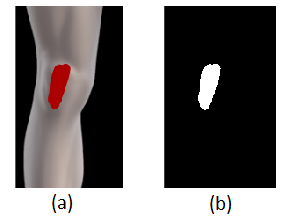
\includegraphics[width=0.8\textwidth]{figures/cropbin7}
\caption{(a) Original pain map and (b) image consisting of a binary matrix where white color represents the pain pixels.}
\label{fig:cropbin7}
\end{figure}

\noindent
An illustration of this data representation is created to convey how the data is assembled and transferred to the model. The illustration is shown by figure \ref{fig:binmatrix}.

\begin{figure} [H]
\centering
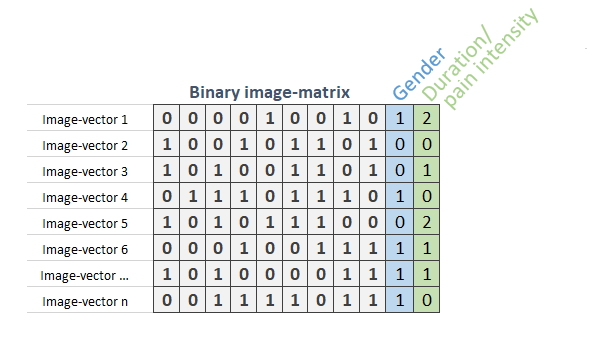
\includegraphics[width=1\textwidth]{figures/binaryimagematrix}
\caption{An illustration of the matrix of the morphology data representation. The matrix consist of image-vectors for each subjects where the two last column indicate the appurtenant gender and either duration or pain intensity. The image-vectors has a length equal to the number of pixel in the pain maps.}
\label{fig:binmatrix}
\end{figure}


\subsection{Regions}
The second representation of the data is a matrix consisting of vectors with 20 values which indicate pain in relation to knee regions. 
The knee regions shown in figure \ref{fig:atlas} are converted into a matrix consisting of 20 values, which represent each knee regions. This matrix is superimposed to the binary image of the pain map, which results in a matrix with pain represented in each knee region. In figure \ref{fig:binregions} is there two illustrations of regions with different values (figure \ref{fig:binregions}(a)) and the pain in the specific regions (figure \ref{fig:binregions}(b)).

\begin{figure} [H]
\centering
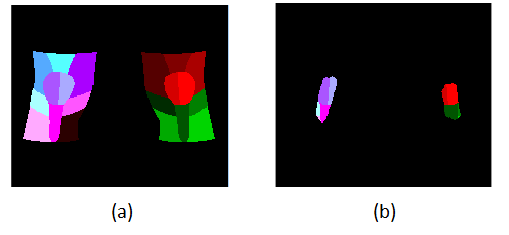
\includegraphics[width=0.8\textwidth]{figures/binregions}
\caption{(a) Knee regions and (b) pain in the specific regions.}
\label{fig:binregions}
\end{figure}

\noindent
After superimposing the two matrices, knee regions and pain, the number of pixels in each active knee region is found. This number is compared to the total number of pixels that are in each knee region, so knee regions with less than 15 \% pain are excluded. WHY 15\%. As an result is a vector with 20 values created. This data representation is implemented the same way as the first representation, figure \ref{fig:binmatrix}. The only different is that the length of the image-vectors respond to the 20 regions, and therefore only is 20 values in this data representation. 


\subsection{Superimposed morphology and regions}
The third representation of the data is a matrix consisting of subject's pain divided into the knee regions.
\noindent
In this representation the superimposed matrix from the second data representation is used. Since the data representation should reflect the morphology of the pain and divide the pain into the different knee regions is one-hot encoding used. One-hot encoding is a way to separate categorical data into binary data \citep{Harris2012}. This means that the 20 values for each knee region do not have a correlation. After one-hot encoding the superimposed matrix consists of 20 layers where each layer represents a knee region.

